\documentclass[a4paper,11pt]{article}
%Premeable
	%Chinese
	\usepackage[UTF8,fontset=fandol]{ctex}
	\xeCJKsetup{underdot = {
		boxdepth=0pt, format=\huge, depth=.4em
	}}
	\usepackage[datesep=/]{datetime2}
	\DeclareTextFontCommand{\textbf}{\sffamily}
%Presenting
	\usepackage[table]{xcolor}
	\usepackage{graphicx}
	\usepackage[font={sf}]{caption}
	\usepackage[above]{placeins}
	\usepackage{float,wrapfig}
	\usepackage{tabularx,array,booktabs,multirow,bigstrut}
	\newcolumntype{C}[1]{>{\hsize=#1\hsize%
		\centering\arraybackslash}X}
	\newcommand{\minitab}[2][l]{%
		\begin{tabular}{#1}#2\end{tabular}}
%MathSetting
	\let\latexointop\ointop
	\usepackage{amsmath,bm,amssymb,esint,extarrows}
	\usepackage{upgreek,textcomp,mathrsfs}
	\usepackage[only,sslash]{stmaryrd}
	\usepackage{nicefrac,eqnarray}
%	\usepackage{amsthm}
	\usepackage{mathtools,physics,siunitx}
	\usepackage{stackengine,titling,varwidth}
	\usepackage{tikz}
	\usepackage{resizegather,empheq}
	\usetagform{default}
	\usepackage{calligra,fourier-orns}
	% Keep \oint unchanged by esint
	\let\ointop\undefined
	\let\ointop\latexointop
	% Define a scriptr 
	\DeclareMathAlphabet{\mathcalligra}{T1}{calligra}{m}{n}
	\DeclareFontShape{T1}{calligra}{m}{n}{<->s*[2.2]callig15}{}
	\newcommand{\scriptr}{\mathcalligra{r}\,}
	\newcommand{\rvector}{\pmb{\mathcalligra{r}}\,}
	% Useful shorthand
	\DeclarePairedDelimiter\ave{\langle}{\rangle}
	\newcommand\inlineeqno{\stepcounter{equation}\ (\theequation)}
	\newcommand{\sinc}{\operatorname{sinc}}
	\newcommand{\mbb}[1]{\mathbb{#1}}
	\newcommand{\mrm}[1]{\mathrm{#1}}
	\newcommand{\mcal}[1]{\mathcal{#1}}
	% Scaling and positioning
	\newcommand\scalemath[2]{\scalebox{#1}{\mbox{\ensuremath{\displaystyle #2}}}}
	\newcommand\raisemath[2]{\raisebox{#1\depth}{${#2}$}}
	\empheqset{box=\bbox}
	% Presenting
	\newcommand*\bbox[1]{\fbox{\hspace{1em}\addstackgap[5pt]{#1}\hspace{1em}}}
	\sisetup{%
		redefine-symbols=false,%
		separate-uncertainty=true,%
		range-phrase=\,\textasciitilde\,,%
		arc-separator = \,}
	\allowdisplaybreaks[2]
%ParagraphSetting
	\setlength{\parskip}{.3\baselineskip}
	\usepackage[defaultlines=2,all]{nowidow}
	\postdisplaypenalty=50
%PageSetting
	\usepackage[colorlinks=true,linkcolor=blue]{hyperref}
	\usepackage[vmargin={4cm,5cm},hmargin=3cm,%
		footnotesep=\baselineskip]{geometry}
	\usepackage[bottom]{footmisc}
	\usepackage{changepage}
	% Autoref names
	\renewcommand{\tableautorefname}{\tablename}
	\renewcommand{\figureautorefname}{\figurename}
	% List settings
	\usepackage{enumitem}
	\setlist{itemsep=0pt,topsep=0pt,labelindent=\parindent,leftmargin=0pt,itemindent=*}
	% Some redefined lengths
	\setlength{\headsep}{2.2cm}
	\setlength{\droptitle}{-2.2cm}
	\setlength{\footnotesep}{3\parskip}
	% Header
	\usepackage{fancyhdr,lastpage}
	\pagestyle{fancy}
	\fancyhf{}
	\cfoot{--\ \thepage\,/\,\pageref{LastPage} \ --}
	\renewcommand{\headrulewidth}{0.1pt}
	\renewcommand{\headrule}{
		\vbox to 2pt{
		\hbox to \headwidth{\dotfill}\vss}}
	% Separator
	\newcommand{\newparagraph}{\pagebreak[3]\noindent%
		\hfil
		~\raisebox{-4pt}[10pt][10pt]{\decofourright~~~~~~~~\decofourleft}~ %
		\par
	}
%TitleSettings
	\pretitle{\begin{center}}
	\posttitle{\par\end{center}\vspace{-6mm}}
	\predate{}
	\postdate{\vspace{-4mm}}
%Header
	\lhead{%
		
\includegraphics[height=3.2em]{../PKUPhy}
		\vspace{-3ex}
		}
	\rhead{%
		\itshape\small
		\begin{tabular}{rr}
			\multicolumn{2}{r}{Bryan} \\[.3em]
			学号:   & 1500000000 \\[.2em]
			实验日期:& 2017/05/12 \\[.5em]
		\end{tabular}\hspace{-1em}
		}
%Title
	\title{\textit{\large 实验二十四}\\[2mm]
		\textbf{\LARGE 闪光法测定不良导体的热导率}}
	\author{\textit{Bryan} 1500000000}
	\date{}
%Miscellaneous
	\newcommand{\tabindent}{\hspace{2em}}
%FourierTransform
	\newcommand{\ftransform}{\xlongrightarrow{\ \mathscr F\ }}
	\newcommand{\iftransform}{\xlongrightarrow{\ \mathscr F^{-1}\ }}

\begin{document}
\maketitle
\thispagestyle{fancy}
\section{数据及处理}
\subsection{样品的密度和比热容}
	通过测量样品的质量和几何尺寸,计算得到其密度。测定数据及结果如下:
	\begin{table}[H]
	\centering\caption{样品密度测定数据表}
	\small
	\begin{tabularx}{.85\linewidth}{C{1} *6{C{.8}}}
	\toprule
		\textbf{胶布板} &
		$L / \si{\cm}$ &
		$W / \si{\cm}$ &
		$H / \si{\mm}$ &
		$V / \si{\cm^3}$ &
		$m / \si{\g}$ &
		$\rho / \si{\g\cdot\cm^{-3}}$ \\
	\midrule
		1     & 9.90  & 9.89  & 3.080 &       &       &  \\
		2     & 9.91  & 9.88  & 3.085 &       &       &  \\
		3     & 9.90  & 9.90  & 3.075 &       &       &  \\
		均值    & 9.90  & 9.89  & 3.080 & 30.17 & 41.02 & 1.36 \\
	\bottomrule
	\end{tabularx}
	
	\vspace{3ex}
	\begin{tabularx}{.85\linewidth}{C{1} *6{C{.8}}}
	\toprule
		\textbf{瓷砖} &
		$L / \si{\cm}$ &
		$W / \si{\cm}$ &
		$H / \si{\mm}$ &
		$V / \si{\cm^3}$ &
		$m / \si{\g}$ &
		$\rho / \si{\g\cdot\cm^{-3}}$ \\
	\midrule
		1     & 10.00 & 10.02 & 0.90  &       &       &  \\
		2     & 9.95  & 10.00 & 0.85  &       &       &  \\
		3     & 10.05 & 10.01 & 0.88  &       &       &  \\
		均值    & 10.00 & 10.01 & 0.88  & 87.75 & 214.58 & 2.45 \\
	\bottomrule
	\end{tabularx}
	\end{table}\noindent%
	样品的比热容$c$和被照射样品的厚度$h$均已事先测定,有:
	\begin{table}[H]
	\centering\caption{样品的已知参量表}
	\small
	\begin{tabularx}{.5\linewidth}
		{@{\hspace{1.5em}} p{5em} *2{S[table-format=1.2e-1]}}
	\toprule
		\textbf{样品} &
		$c / \si{\J\cdot\kg^{-1}\kelvin^{-1}}$ &
		$h / \si{\m}$ \\
	\midrule
		胶布板   & 1.04e3 & 3.02E-03 \\
		瓷砖     & 0.71e3 & 3.03E-03 \\
	\bottomrule
	\end{tabularx}
	\end{table}
	
\subsection{温升曲线的特征量}
	记录闪光照射样品后的温升曲线,记录初始温度$T_0$, 最高温度$T_M$, 计算
		$T_{1/2} = \frac{1}{2}\pqty{T_0 + T_M}$, 读取对应的时间$t_{1/2}$, 
	从而得到热导率:
	\begin{equation}
		\lambda = \frac{1.38}{\pi^2}\,\frac{\rho c h^2}{t_{1/2}}
	\end{equation}
	可利用每次测定结果分别计算$\lambda$, 也可利用修正散热后特征时间的均值$\bar{t}_{1/2}$代入计算,结果总结如下。
	\begin{table}[H]
	\centering\caption{胶布板热导率测定数据表}
	\small
	\begin{tabularx}{.95\linewidth}{C{.6} C{1} *4{C{.4}} C{1}}
	\toprule
		多次测量 &
		\footnotesize 散热修正 / \si{\kelvin\cdot\s^{-1}} &
		$T_0 / \si{\kelvin}$ &
		$T_M / \si{\kelvin}$ &
		$T_{1/2} / \si{\kelvin}$ &
		$t_{1/2} / \si{\s}$ &
		\footnotesize $\lambda / \si{\watt\cdot\m^{-1}\K^{-1}}$ \\
	\midrule
		1     & 0     & 0.7987 & 1.1689 & 0.9838 & 6.7587 & 0.267 \\
	\midrule
		1'    & 0.001243 & 0.7987 & 1.1949 & 0.9968 & 6.8973 & 0.261 \\
		2'    & 0.001399 & 0.7326 & 1.0898 & 0.9112 & 7.0282 & 0.257 \\
		3'    & 0.001258 & 0.6922 & 1.1477 & 0.9199 & 6.9336 & 0.260 \\
		$t_{1/2}$均值   & 0.001300 &  --   &  --   &  --   & 6.9530 & \bfseries 0.259 \\
		$\lambda$均值 & 0.001300 &  --   &   --  &   --  &  --   & \bfseries 0.259 \\
	\bottomrule
	\end{tabularx}
	\end{table}
	
	首先,看已加粗的最终测定数据,可见先计算$\bar{t}_{1/2}$再代入得$\lambda$, 和先分别计算$\lambda$再平均得$\bar{\lambda}$, 这两种方式得到的测定值没有显著不同。
	
	此外,将散热修正前后的$\lambda$测定值标注在数轴上,比较如下:
	\begin{figure}[H]
	\centering
	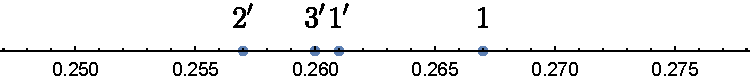
\includegraphics[width=.8\linewidth]{lineplot}
	\caption{散热修正对$\lambda$测定值的影响}
	\end{figure}\noindent%
	可见散热修正后的各测定值基本一致,而散热修正前的测定值显著偏大,这表明散热修正是十分必要的。
	
	对瓷砖样品重复上述步骤,同时调整并记录每一组数据的\textbf{采样时间},结果如下。
	\begin{table}[H]
	\centering\caption{瓷砖热导率测定数据表}
	\small
	\begin{tabularx}{\linewidth}
		{C{.55} C{.75} C{1} *4{C{.35}} C{.75}}
	\toprule
		\footnotesize 多次测量 &
		\footnotesize 采样时间 / \si{\s} &
		\footnotesize 散热修正 / \si{\kelvin\cdot\s^{-1}} &
		$T_0 / \si{\kelvin}$ &
		$T_M / \si{\kelvin}$ &
		$T_{1/2} / \si{\kelvin}$ &
		$t_{1/2} / \si{\s}$ &
		\footnotesize $\lambda / \si{\watt\cdot\m^{-1}\K^{-1}}$ \\
	\midrule
		1     & 38  & 0     & 0.2013 & 0.5730 & 0.3087 & 4.0529 & 0.550 \\
	\midrule
		1'    & \bfseries 38  & \bfseries 0.001506 & 0.2011 & 0.6071 & 0.4041 & 4.3090 & 0.517 \\
		2'    & \bfseries 33    & \bfseries 0.001350 & 0.2664 & 0.6644 & 0.4655 & 4.2150 & 0.529 \\
		3'    & \bfseries 30    & \bfseries 0.001439 & 0.2283 & 0.6433 & 0.4358 & 4.1984 & 0.531 \\
		$t_{1/2}$均值   &       & 0.001432 &       &       &       & 4.2408 & \bfseries 0.526 \\
		$\lambda$均值 &       & 0.001432 &       &       &       &       & \bfseries 0.526 \\
	\bottomrule
	\end{tabularx}
	\end{table}
	
	在瓷砖样品的三次测定中,单调地减小了采样时间,但相应的散热修正系数并不是单调变化的,且差距不很显著;由此猜想,采样时间对软件自动散热修正的影响有限;对自动散热修正影响最为显著的可能是热噪声及其他因素。
\section{分析与讨论}
\subsection{关于散热修正的进一步分析}
	软件通过记录温升曲线的峰值和后续散热曲线的终点,以这两点确定的直线斜率为散热修正系数$k$, 进一步令$T' = T - kt$得到散热修正后的曲线。
	
	下面考察这一过程的合理性。首先,考虑理想化的模型,满足绝热条件,记温变曲线为$T(x,t)$, 且脉冲对初始温度的影响为:
	\begin{equation}
		T(x,0) = \delta(x)
	\end{equation}
	为便于讨论,可将有关参量无量纲化,如取样品厚度$h = 1$; 记热扩散率为$\alpha$, 则有:
	\begin{equation}
		T(1,t) = 1 + 2\sum_{n=1}^{\infty}
			(-1)^n e^{-n^2\pi^2\tau},\quad
		\tau = \alpha t,\ 
		\lambda = \alpha\rho c
	\end{equation}
\pagebreak
	
	相应地,脉冲在介质中的传导如下所示:
	\begin{figure}[H]
	\centering
	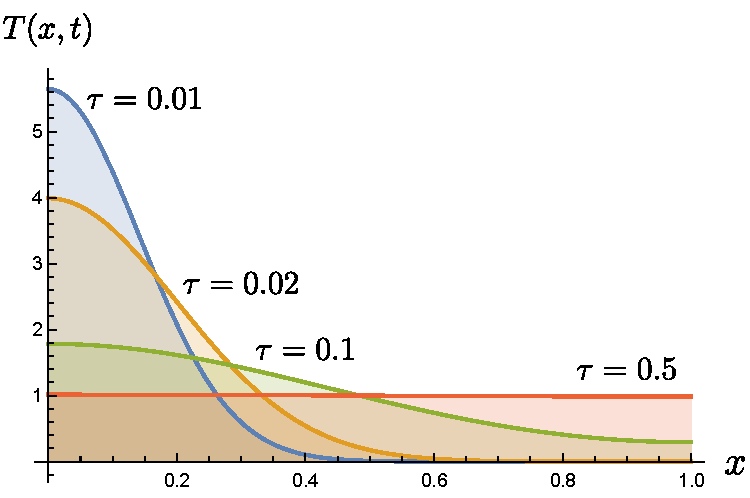
\includegraphics[width=.6\linewidth]{heatConducting.pdf}
	\caption{热脉冲在一维介质中的传导}
	\end{figure}\noindent%
	由上图可见,热流传递的过程很像一个中心位于原点的不断扩散的\textbf{高斯波包}。
	
	若考虑样品在前后两面的散热,则可以将边界$\Sigma$上的条件修正为:
	\begin{equation}
		\pqty{\pdv{T}{n} + hT}_\Sigma = 0
	\end{equation}
	其中$h$待定,它表征了散热的强度;这里忽略了前后表面$h$值的不同。此时,要获得方程的解析解就较为困难了,但可以考虑用数值方法求解方程。受到上述导热图像的启发,可以取初始温度分布为高斯型分布:
	\begin{figure}[H]
	\centering
	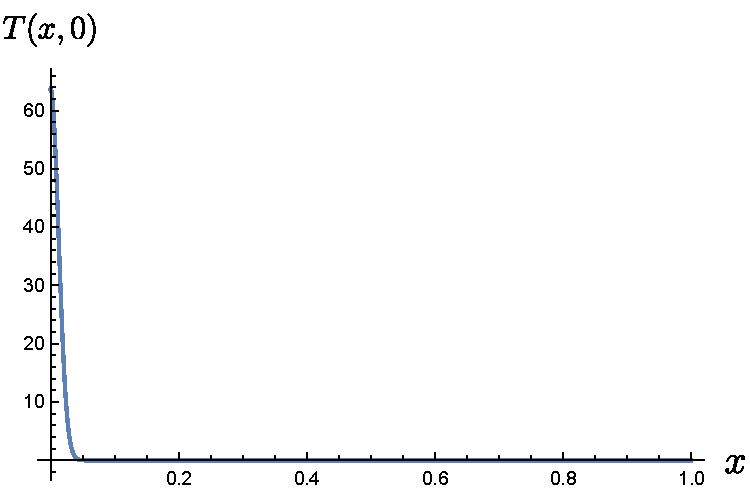
\includegraphics[width=.6\linewidth]{initCondition.pdf}
	\caption{初始温度分布曲线}
	\footnotesize
	\textit{采用\texttt{Mathematica}内置的正态分布函数:}
	\texttt{PDF[HalfNormalDistribution[a], x] /. \{a -> 55\}}
	\end{figure}
	
	数值求解热传导方程,首先比较$h=0$情况下数值解与解析解的差异:
	\begin{figure}[H]
	\centering
	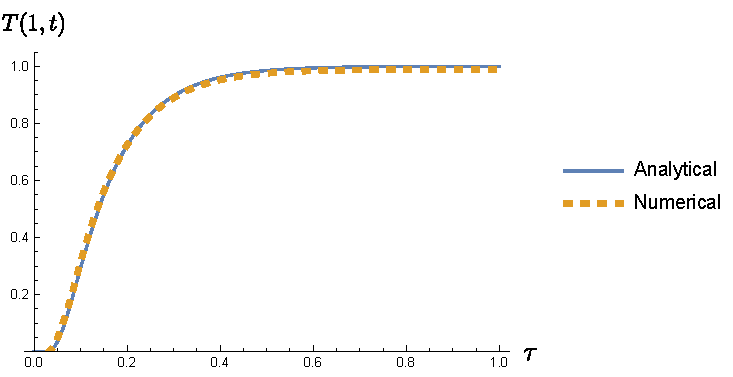
\includegraphics[height=.35\linewidth]{numericComp.pdf}
	\caption{绝热情形数值解(Numerical)与解析解(Analytical)的比较}
	\end{figure}\noindent%s
	可见两者基本一致;进一步对$h = 0.03$求解方程,可得:
	\begin{figure}[H]
	\centering
	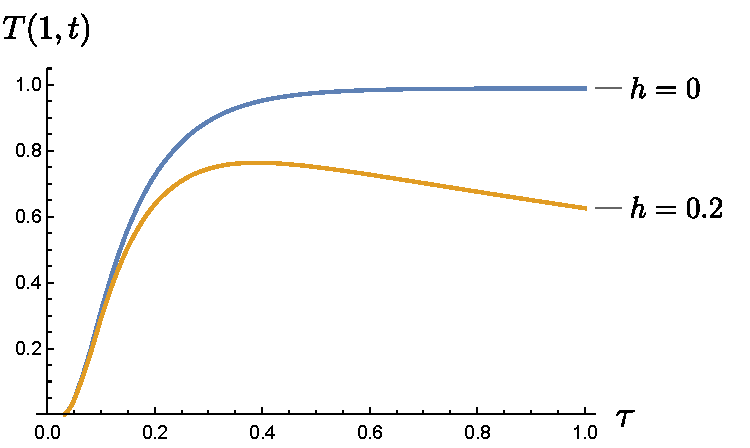
\includegraphics[height=.35\linewidth]{solWithLoss.pdf}
	\caption{绝热情形与考虑散热情形的数值解之比较}
	\label{fig:sealed_vs_lost}
	\end{figure}
	
	可见,数值解与实测曲线的模式完全一致。事实上,对胶布板,经过线性缩放调整后,可使数值计算结果与温变曲线基本吻合:
	\begin{figure}[H]
	\centering
	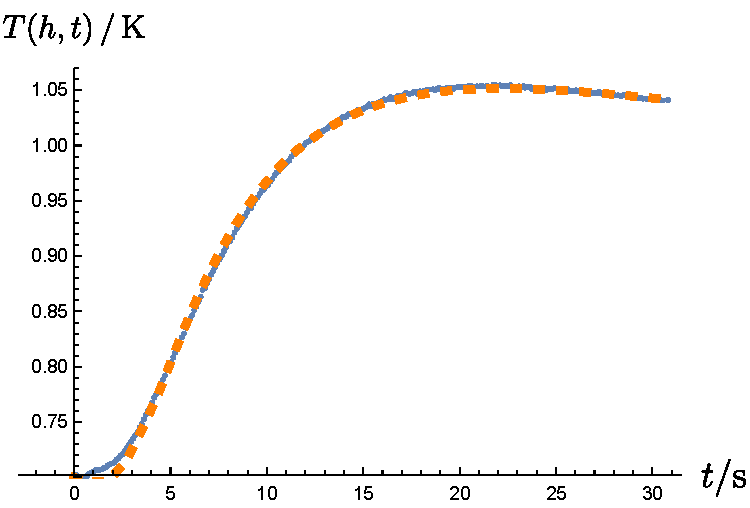
\includegraphics[height=.35\linewidth]{datFit.pdf}
	\caption{实测温变曲线与数值计算结果(虚线)之比较}
	\end{figure}
	
	在此基础上,分析散热对温变曲线的影响;\autoref{fig:sealed_vs_lost} 中两条曲线的差异如下:
	\begin{figure}[H]
	\centering
	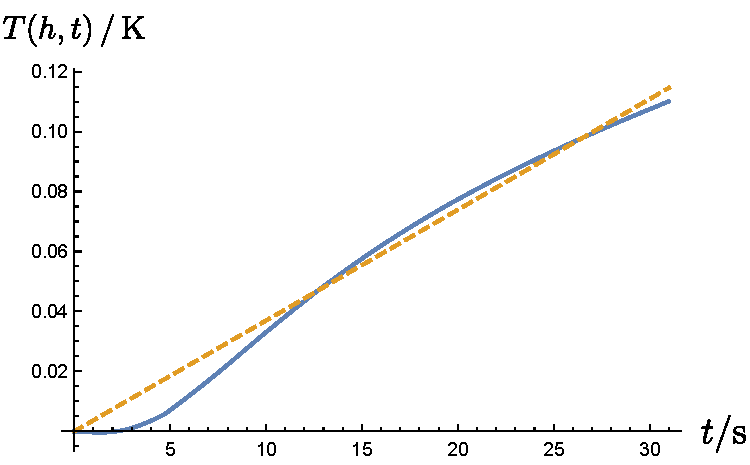
\includegraphics[height=.35\linewidth]{linearCorrection.pdf}
	\caption{散热修正的数值计算结果}
	\end{figure}\noindent%
	可见温度差异关于时间确实具有不错的线性特征;在曲线上等间隔取样,计算可得相关性系数约为 \num{.994854}. 
	
	由此可见,对全过程进行线性散热修正是可行的;$k$可以通过实测曲线后段的散热部分之切线、割线斜率来估计。但由上述图像可知,这种办法估计出的散热系数$k$将略微偏小。实际上,据牛顿冷却定律,后期的温度应当是指数下降的,从而修正曲线将渐趋平缓,直至为零。
	
	可以手动取点以实现散热修正;对每个样品的第3组原始数据,在散热曲线上取点,计算相关性系数$r$和$k$, 可得:
	\begin{table}[H]
	\centering\caption{手动散热修正数据表}
	\small\vspace{-5ex}
	\flushleft\qquad\ \textbf{胶布板}\par\vspace{2ex}\centering
	\begin{tabularx}{.9\linewidth}
		{C{.6} | *6{C{.8}} | *2{C{1}}}
	\toprule
		$t / \si{\s}$ &
		22.5666 & 23.0778 & 23.8947 & 25.1016 & 25.6550 & 26.4298 &
		$r$ & $k / \si{\kelvin\cdot\s^{-1}}$ \\
	\midrule
		$T / \si{\kelvin}$ &
		1.1201 & 1.1196 & 1.1182 & 1.1168 & 1.1154 & 1.1139 & 0.993278 & 0.001585 \\
	\bottomrule
	\end{tabularx}
	
	\flushleft\qquad\ \textbf{瓷砖}\par\vspace{2ex}\centering
	\begin{tabularx}{.9\linewidth}
		{C{.6} | *6{C{.8}} | *2{C{1}}}
	\toprule
		$t / \si{\s}$ &
		20.5012 & 21.9686 & 23.6138 & 25.0367 & 26.5486 & 28.1938 &
		$r$ & $k / \si{\kelvin\cdot\s^{-1}}$ \\
	\midrule
		$T / \si{\kelvin}$ &
		0.6366 & 0.6351 & 0.6335 & 0.6324 & 0.6305 & 0.6285 & 0.997368 & 0.001034 \\
	\bottomrule
	\end{tabularx}
	\end{table}
	
	可见,线性良好;但由于取点位置的不同,给出的$k$值与自动散热修正的不尽相同,但两者数量级一致。
\subsection{误差分析}
	$\lambda$测定值的精确程度强烈依赖于$t_{1/2}$的精度。由上述实验数据可见,$t_{1/2}$值容易受到两大因素的影响,分别是\textbf{散热问题}和\textbf{热噪声}。
	
	根据前面的讨论可知,散热问题可以通过修正的办法极大地改善,从而使得$T_M$测定值更加精确,进而导致$T_{1/2}, t_{1/2}$的读出值更加准确。热噪声的影响可以通过多次测量取均值的方法尽可能地消除。
\section{思考}
\subsection{实验装置和测定过程应当满足的条件}
	由上述分析可见,此实验的理论模型在一维导热、边界绝热、一侧输入单次脉冲式热流的前提下成立。
	
	实验过程中,取薄圆片状样品,令瞬时闪光均匀照射其表面,且控制光线垂直与表面,从而使得样品一侧极薄层内均匀吸热。样品很薄,从而有效控制了侧面的散热,保证了一维热流条件;控制温升也有效地减小了散热的影响。
	
	此外,$T_0,T_M$均对应平衡态,因此应当待装置充分冷却时开始测量;测量过程中尽量不要干扰装置,以免影响传热或数据采集。
\subsection{对测温传感器的要求}
	测温传感器应当充分地小,这可使绝热边界条件不被破坏;同时,较小尺寸的传感器具有较小的热容,猜想这可使其较快达到与待测环境一致的温度,从而导致测温响应及时。
\subsection{初始温度和时间的测定}
	通过合理设计实验电路,可使闪光时刻与采样时间零点重合,从而$t = 0$便是时间起点,相应的温度便是所需数据$T_0$. 
\subsection{相应物理量的意义}
	$t_{1/2}$是实验中最为关键的测定值之一,它可以看作该样品中热传导的\textit{特征时间}; 相应地,$\lambda$表征了传热的速率, 自然便有$\lambda\propto\frac{1}{t_{1/2}}$. 
	
	同时,$c$是样品的比热容,它给出了温度变化和吸热量的关系,但与传热速率无关;由于实验中测温比测热量来得方便的多,因此通过测定温度变化,再乘以比例系数$c$得到热量。自然有$\lambda\propto c$. 
\subsection{脉冲光对记录装置的干扰}
	实验中可见,脉冲光照射后一瞬间,温变曲线上可见一微小但明显的尖峰。首先,传感器被样品、样品盒包裹,并没有直接受到闪光照射,且传热时间远大于尖峰的时间尺度,因此这一现象不可能源于热传导。
	
	由于闪光由瞬间大电流产生,猜想这一尖峰源于电磁干扰;可以通过恰当的屏蔽手段控制其对采集数据的影响。
	
	\vfill\noindent\itshape\footnotesize
	\hfill Last edited: \today\ \copyright\ Bryan
\end{document}